%%%%%%%% FInk — IE412 AI for Finance (2026 Spring) final project %%%%%%%%
\documentclass{article}

\usepackage{microtype}
\usepackage{graphicx}
\usepackage{booktabs}
\usepackage{hyperref}
\usepackage{url}

\newcommand{\theHalgorithm}{\arabic{algorithm}}

% Camera-ready / named version (this is a course submission that shows the author).
\usepackage[accepted]{icml2026}

\usepackage{amsmath}
\usepackage{amssymb}
\usepackage{amsthm}
\usepackage[capitalize,noabbrev]{cleveref}

\theoremstyle{plain}
\newtheorem{proposition}{Proposition}

\icmltitlerunning{FInk: Creator-Contract Financial-Risk Review}

\begin{document}

\twocolumn[
  \icmltitle{FInk: An On-Device, Evidence-Gated Retrieval System for\\
    Financial-Risk Review of Creator Contracts}

  \icmlsetsymbol{equal}{*}

  \begin{icmlauthorlist}
    \icmlauthor{Seonuk Kim}{ie}
  \end{icmlauthorlist}

  \icmlaffiliation{ie}{Department of Industrial Engineering, UNIST, Ulsan, Korea}
  \icmlcorrespondingauthor{Seonuk Kim}{seonuk.kim@unist.ac.kr}

  \icmlkeywords{financial NLP, retrieval-augmented generation, on-device,
    decision support, creator economy, contract analysis}

  \vskip 0.3in
]

\printAffiliationsAndNotice{}

\begin{abstract}
Creators sign revenue-sharing contracts under time pressure and with little
financial training, and the clauses that move the most money---settlement basis,
deductions, recoupment, payment timing---are the easiest to miss. Making review
\emph{available} is not the same as getting it \emph{used}: a large field study
found that the people who most need unbiased financial advice are the least
likely to take it. We present FInk, an on-device assistant that reads a creator's
contract, detects financial risk across nine cash-flow categories, grounds each
flag in a curated corpus of official Korean standard contracts and counseling
casebooks through BM25 retrieval, and returns a prioritized review: a
$0$--$100$ review-attention score, a recommended review effort, and ranked,
source-cited findings, with a local chatbot for follow-up questions. An evidence
gate lets only officially grounded clauses raise the score, so unverified signals
inform questions but never inflate risk. On synthetic, sanitized fixtures a
rule\,+\,model hybrid gives the best risk detection (macro-F1 $0.92$) while
keeping false positives low, retrieval returns the correct authority tier and is
consistent across Korean and English queries, and a decision-aware ordering
covers more financial exposure within a small reading budget than a severity-only
baseline; the whole pipeline runs locally with no network calls. FInk is decision
support for what to check before signing, not legal advice or a verdict. FInk is
available at \url{https://fink.seonukkim.com}.
\end{abstract}

\section{Introduction}
\label{sec:intro}

\begin{figure*}[t]
  \centering
  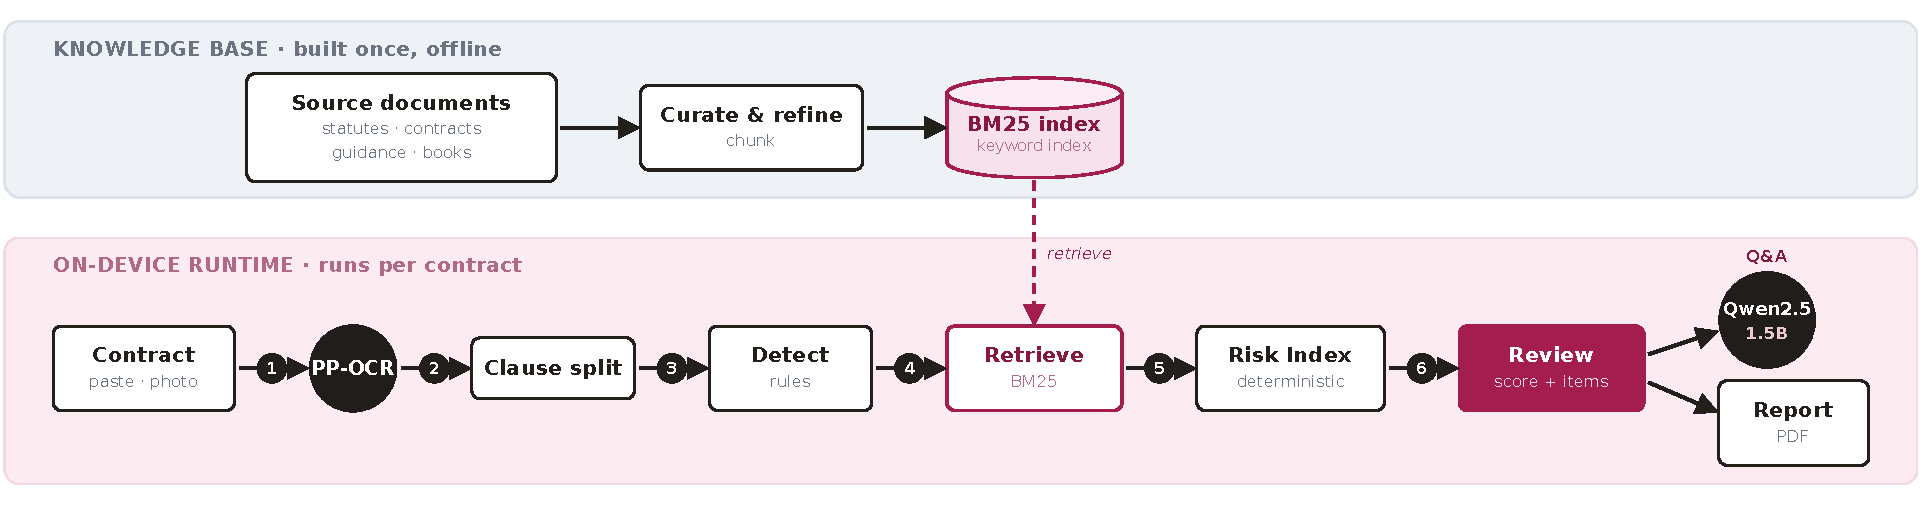
\includegraphics[width=\textwidth]{figures/pipeline.pdf}
  \caption{FInk pipeline. An offline knowledge base of curated Korean sources is
  built once and indexed for retrieval. At runtime, per contract and on device,
  the text is split into clauses, financial risk is detected, each signal is
  grounded by BM25 retrieval against the knowledge base, and a deterministic
  review-attention score and ranked findings are produced; a small local model
  answers follow-up questions, and the review exports as a brief.}
  \label{fig:pipeline}
\end{figure*}

The creator economy runs on contracts. Webtoon artists, illustrators, and writers
sign agreements that fix how revenue is split, what is deducted before they are
paid, when the money actually arrives, and who keeps the secondary rights. Those
terms decide a creator's real cash flow, often more than the headline rate does.
The people signing them usually have no finance or legal background and little
time before a deadline.

The clauses with the largest financial consequence are also the easiest to skip.
A recoupment clause, a vague deduction basis, or a ninety-day settlement delay can
quietly move a large share of income, yet each sits among many routine terms and
reads as boilerplate. Signing is close to irreversible: afterward, renegotiation
is hard. Professional review exists, but offering advice is not the same as people
using it. In a field study of roughly eight thousand retail investors, the clients
who most needed unbiased advice were the least likely to obtain it, and the few
who did barely followed it; the authors conclude that unbiased advice is necessary
but not sufficient~\citep{bhattacharya2012advice}. A tool that lowers the cost of
\emph{knowing what to ask before signing} targets that uptake gap, not only the
availability gap. Privacy makes the problem sharper: a draft contract is sensitive
personal and business information, and uploading it to a cloud service to be read
is itself a disclosure many creators would rather avoid.

We present FInk, an on-device assistant for financial-risk review of creator
contracts. FInk reads a pasted or photographed contract, splits it into clauses,
detects financial risk across nine cash-flow categories---from settlement
transparency to production-cost burden---and grounds each flag by retrieving
supporting passages from a curated corpus of official Korean standard contracts
and counseling casebooks. It then reports a prioritized review: a $0$--$100$
review-attention score, a three-level recommended review effort, and a ranked list
of findings, each naming its clause and the sources behind it. A small on-device
chat model answers follow-up questions over the same grounded material, and the
review can be saved as a one-page brief.

The choice that holds FInk together is an evidence gate. Only clauses supported by
official, score-eligible sources contribute to the score; signals taken from
practice books or unverified text can still raise a question, but they never raise
the risk number. The score is a deterministic function rather than a learned
black box: a saturating per-category severity combined into a bounded index, with
weights drawn from standard risk-assessment practice. This keeps FInk conservative
by construction and keeps its output readable as a review priority, not a ruling.

Real creator contracts are private, so we evaluate on synthetic, sanitized
fixtures and report every number as measured-on-fixture rather than a generalized
claim. On these fixtures a rule\,+\,model hybrid detects financial risk best while
keeping false positives low; retrieval returns the correct authority tier and
agrees across Korean and English queries; a decision-aware ordering covers more
financial exposure within a small reading budget than a severity-only baseline;
and the pipeline runs locally with no outbound calls. Our contributions are:

\begin{itemize}
  \item a financial-risk taxonomy for creator contracts and an evidence-gated
        scoring design that separates \emph{what to review} from \emph{what is
        verified}, so unverified signals never inflate the risk score;
  \item an on-device retrieval-augmented pipeline that grounds creator-contract
        risk in official Korean financial and legal sources and answers follow-up
        questions without the contract leaving the device; and
  \item a decision-focused evaluation, on synthetic fixtures, that measures
        whether FInk's ordering helps a creator cover financial exposure under a
        limited reading budget, not only whether clauses are classified correctly.
\end{itemize}

\section{Related Work}
\label{sec:related}

\paragraph{Retrieval-augmented generation for financial documents.}
Retrieval-augmented generation answers from retrieved evidence rather than from
parameters alone~\citep{lewis2020rag}, with BM25~\citep{robertson2009bm25} and
dense retrieval~\citep{karpukhin2020dpr} as the standard retrievers. Financial
question answering has moved toward realistic retrieval. FinDER shows that real
financial queries are short and jargon-heavy, so the hard part is retrieval rather
than reading a context that has already been handed to the
model~\citep{choi2025finder}; FinAgentBench frames retrieval as multi-step, first
choosing the document type and then the passage~\citep{choi2025finagentbench}.
FInk applies evidence-gated retrieval to a different financial document, the
creator's own contract, over a small curated Korean corpus, and runs the whole
loop on device, where a heavy dense retriever is impractical and a sparse BM25
index is a deliberate fit rather than a fallback.

\paragraph{Decision-focused and responsible financial AI.}
Decision-focused learning argues that a predictor should be judged by the decision
it supports, not only by predictive error~\citep{elmachtoub2022spo}. Evaluation of
financial language models is fragile: \citet{kong2026bias} catalog biases---among
them narrative and objective bias---that let fluent, confident output look like a
result, and warn against treating persuasion as evidence. And availability is not
uptake: unbiased advice was necessary but not sufficient in the field study above
\citep{bhattacharya2012advice}. FInk is decision-focused in spirit---it orders
findings by financial exposure and is evaluated on whether that ordering covers
more exposure under a reading budget---but it does not train end to end through an
optimizer. The evidence gate and the explicit not-a-verdict framing are our
response to the narrative and objective biases that make confident financial
outputs hard to trust.

\paragraph{On-device and privacy-preserving document AI.}
Small instruction-tuned models such as Qwen2.5~\citep{qwen2024report} and
lightweight OCR such as PP-OCR~\citep{du2020ppocr} make local document
understanding workable on commodity hardware. Earlier on-device work usually
targets latency or cost. FInk instead treats locality as the privacy property
itself---a draft contract never leaves the device---and accepts the resulting
capability ceiling, a $1.5$B chat model, as a design constraint rather than a
limitation to hide.

\section{Design Goals}
\label{sec:goals}

The problem and the responsible-AI concerns above give five goals; every later
design decision points back to one of them.

\begin{description}
  \item[G1. Decision support, not a verdict.] The output is a review priority and
    a set of questions to ask, never a ruling on legality, fraud, validity,
    fairness, or guaranteed loss.
  \item[G2. Evidence-gated scoring.] Only official, score-eligible sources can
    raise the score. Unverified signals inform questions only.
  \item[G3. On device by default.] Ingestion, OCR, retrieval, scoring, and the
    chat model run locally; no contract text leaves the device.
  \item[G4. Prioritized and actionable.] The creator receives an ordering---what
    to check first and why---that fits a small reading budget, plus a portable
    brief.
  \item[G5. Korean-canonical and bilingual.] Korean source text is canonical;
    English is a retrieval and reading aid, marked as generated and not an
    equivalent legal reading.
\end{description}

\section{System}
\label{sec:system}

FInk has two phases (\cref{fig:pipeline}): an offline knowledge base built once,
and an on-device runtime that runs per contract.

\subsection{Knowledge base and authority tiers}
The knowledge base is curated from real Korean sources. Official material---sector
standard contracts, official contracting guides, and public counseling
casebooks---is score-eligible and tagged by authority tier (A0--A2). Two
creator-law reference books are kept as practice context only: they are distilled
into checkpoint summaries and never contribute to the score (tiers B/C). This
split is the mechanism behind G2. Official sources were preprocessed into Markdown
with Claude Opus 4.8 and the two books with ChatGPT 5.5 Pro, then indexed with
BM25~\citep{robertson2009bm25}; the raw source text is not redistributed, and only
distilled, source-typed summaries are committed. We use BM25 rather than a dense
retriever for three reasons that fit the setting: the corpus is small and curated,
exact Korean legal terms matter, and a sparse index runs on device with no model
to host.

\subsection{From contract to clauses}
The creator pastes text or uploads a photo or PDF. Images and scans pass through
PP-OCR in its Korean configuration~\citep{du2020ppocr}, a small CPU OCR model;
this is one input path, not the focus of the system, and extraction quality is
reported only in the appendix. The text is then segmented into clauses, which are
the unit of detection and grounding.

\subsection{Financial-risk detection}
Each clause is checked against nine cash-flow risk categories, F1--F9: settlement
transparency and audit rights (F1); revenue base and deductions (F2); payment and
cash-flow timing (F3); minimum guarantee and recoupment (F4); intellectual
property and secondary-rights monetization (F5); term, exclusivity, and
opportunity cost (F6); termination, liability, and penalties (F7); scope creep and
production-cost burden (F8); and a residual category (F9). These cover where a
creator-contract clause most often moves cash. Detection runs in three arms: a set
of deterministic rules, a small local classifier, and their union (the hybrid).
We ship the rule arm by default because its decisions are inspectable, and report
all three.

\subsection{Evidence-gated grounding}
For each detected signal, BM25 retrieves supporting passages from the knowledge
base. A signal becomes score-eligible only when an official (A0--A2) source backs
it; otherwise it is kept as a practice-informed note that can raise a question but
not the score. The not-a-verdict stance (G1) is therefore enforced in the data
path, not only in the wording: the score cannot move on text that no official
source supports.

\subsection{Review-attention score}
\label{sec:score}
The score is deterministic. For each category $c$ we map the grounded severity
$x_c$ to a per-category contribution $g_c(x_c)$ that saturates---extra severity
past a point adds little---following standard risk-assessment
practice~\citep{iso31000,iec60812}, and is capped at a category weight $w_c$. The
contributions are summed into a single review-attention index $R=\sum_c g_c(x_c)$
that we keep in $[0,100]$ (\cref{prop:bound}). The weights encode two ideas from
decision theory: the same nominal exposure hurts more when it is less recoverable
or more uncertain, which is risk aversion~\citep{pratt1964risk}, and a single
attention number must trade off several categories that are not directly
comparable, which is multi-attribute value~\citep{keeney1976decisions}. We keep
how strongly a signal is supported separate from how severe it is, in the spirit
of GRADE~\citep{guyatt2008grade}: evidence strength gates eligibility, severity
sets magnitude. The index maps to a three-level recommended review effort---light
check, careful check, or professional review recommended.

\subsection{On-device chat and brief}
A small instruction model, Qwen2.5-1.5B-Instruct in a $4$-bit
build~\citep{qwen2024report}, answers follow-up questions over the grounded
findings. It is prompted to stay on the retrieved material and to keep the review
framing rather than issue a ruling. The review exports as a one-page brief through
the browser's own print path, with no remote document service, consistent with G3
and G4.

\section{Evaluation}
\label{sec:eval}

Real contracts are private, so all evaluation uses synthetic, sanitized fixtures
with a frozen split created once and never edited; tuning used a separate
development split. Every number is measured-on-fixture and is not a generalized
performance claim. We focus the evaluation on the financial-AI parts of the
system; OCR and extraction numbers are in \cref{app:ocr}.

\subsection{Financial-risk detection}
\Cref{tab:detect} compares the three detection arms over F1--F9. The hybrid gives
the best macro-F1 while holding the benign false-positive rate at the rule level;
the model arm alone reaches similar recall but doubles false positives on benign
clauses. On this fixture, combining inspectable rules with the model detects risk
best without becoming trigger-happy on harmless terms.

\begin{table}[t]
  \centering
  \caption{Financial-risk detection over categories F1--F9 (synthetic fixture).
  Higher macro-F1 is better; lower benign false-positive rate (FPR) is better.}
  \label{tab:detect}
  \begin{tabular}{lcc}
    \toprule
    Arm        & Macro-F1 & Benign FPR \\
    \midrule
    Rule only  & 0.83 & 0.25 \\
    Model only & 0.86 & 0.50 \\
    Hybrid     & \textbf{0.92} & 0.25 \\
    \bottomrule
  \end{tabular}
\end{table}

\subsection{Evidence grounding}
On the retrieval fixture, authority-tier correctness is $1.00$: practice (B/C)
sources are never returned as score-eligible, which is the property G2 depends on.
Recall@3 and Recall@5 are both $1.00$, Korean and English versions of a query
resolve to the same evidence ($1.00$ consistency), and cited spans overlap the
gold spans at $0.85$. The gate behaves as designed on the fixture and is
bilingual-consistent.

\subsection{Decision quality}
The decision-focused question is whether FInk's ordering helps a creator cover
financial exposure under a small reading budget, not only whether clauses are
labeled correctly~\citep{elmachtoub2022spo}. We compare an exposure-aware ordering
against a severity-only baseline on a factorial fixture with hidden oracle
exposure weights, and measure oracle exposure coverage at $k$ (OEC@$k$): the share
of total financial exposure captured by the top-$k$ clauses in a given order
(\cref{tab:decision}). Reading in FInk's exposure-aware order covers more exposure
within one to three clauses than reading by severity. When the evidence gate is
on, coverage is lower because only officially grounded clauses are allowed to
count; this is the conservative trade-off the gate is meant to make---it trades
coverage for trustworthiness. In a separate cost-sensitive fixture with a fixed
trigger threshold, the verification trigger recovers $0.67$ of the consequential
clauses at a false-trigger rate of $0.33$, against a synthetic trade-off between
the cost of a missed exposure and the effort of verification; this frames review
as a cost-sensitive decision rather than plain classification, in the spirit of
the course's risk-scoring material.

\begin{table}[t]
  \centering
  \caption{Decision quality: oracle exposure coverage at $k$ (OEC@$k$), higher is
  better, on the synthetic factorial fixture. Exposure-aware ordering covers more
  exposure under a small reading budget than severity-only; the evidence gate
  lowers coverage in exchange for only counting verified clauses.}
  \label{tab:decision}
  \begin{tabular}{llcc}
    \toprule
    Evidence gate & Ordering        & OEC@1 & OEC@3 \\
    \midrule
    Off & Severity baseline & 0.69 & 0.93 \\
    Off & Exposure-aware    & \textbf{0.81} & \textbf{1.00} \\
    On  & Severity baseline & 0.41 & 0.55 \\
    On  & Exposure-aware    & 0.53 & 0.62 \\
    \bottomrule
  \end{tabular}
\end{table}

\subsection{Scoring correctness and runtime}
The scoring module passes all registered formula checks ($13/13$ unit cases and
$10/10$ financial-scenario cases), and the review-attention index stays inside
$[0,100]$ by construction (\cref{prop:bound}). On the runtime fixture, FInk made
zero network attempts across accepted runs, leaked no contract text or file paths
across six log and export surfaces, and ran end to end in well under a second with
a peak memory of tens of megabytes. The on-device privacy property of G3 holds on
the fixture.

\section{Discussion}
\label{sec:discussion}

\paragraph{Decision support, not automation.}
FInk reports a priority rather than a verdict for a reason tied to the task.
Signing is near-irreversible and the money at stake is the creator's own income,
so the failure that matters most is a confident wrong reading the creator acts on.
Keeping the output a review ordering, and routing the strongest cases to
``professional review recommended,'' keeps the person in the decision and uses AI
to lower the cost of knowing what to ask. This is the uptake gap from
\citet{bhattacharya2012advice} addressed at the level of the tool rather than the
advisor.

\paragraph{Evidence-gating as a conservative stance.}
The narrative and objective biases that \citet{kong2026bias} warn about are
exactly what an eager contract-reading model would produce: fluent, confident
readings that look like legal conclusions. The evidence gate is the structural
answer. A signal can raise the score only if an official source backs it, so the
score cannot be inflated by persuasive but ungrounded text. The price is visible
in our own numbers---coverage drops when the gate is on (\cref{tab:decision})---and
we accept it as the cost of not overclaiming.

\paragraph{Privacy against capability.}
Running on device buys privacy and costs capability. A $1.5$B chat model grounded
by retrieval is weaker than a large hosted model, and in practice its free-form
answer quality was the main limit we hit. Retrieval narrows the gap by holding
answers to retrieved evidence, but does not close it. We treat this as the honest
price of G3 rather than something to paper over, and it sets the agenda for future
work: better grounding and calibration for small local models.

\paragraph{What changes for the creator.}
FInk shifts the pre-signing step from ``read everything or read nothing'' to
``read the few clauses that move the most money, with the questions to ask
attached.'' The exported brief carries that into a negotiation.

\section{Limitations}
\label{sec:limitations}

The evaluation is on synthetic, sanitized fixtures; there is no study with real
creators or real contracts, and no number here should be read as generalizing
beyond the fixture. The on-device chat model has a real answer-quality ceiling
that we did not fully calibrate, which we accept as a consequence of G3. The
knowledge base is Korean and centered on webtoon and copyright material; one
intended source, an arts-welfare casebook, was unavailable and is not in the live
knowledge base, so some real risks may go ungrounded. Deterministic detection
misses paraphrases the rules do not anticipate. FInk is a review aid, not a ruling
on legality, fraud, validity, fairness, or loss, and important decisions still
need a professional. As a single-author course project, the depth of the
evaluation matches that scope.

\section{Conclusion}
\label{sec:conclusion}

FInk is an on-device, evidence-gated retrieval-augmented assistant that turns a
creator's contract into a prioritized financial-risk review and answers follow-up
questions, without the contract leaving the device. On synthetic fixtures a
rule\,+\,model hybrid detects financial risk best while staying conservative on
benign clauses, the evidence gate returns the correct authority tier, and a
decision-aware ordering covers more exposure under a reading budget than a
severity baseline. The design keeps the creator in the decision and treats privacy
and conservatism as first-class constraints. The next step is to move from
synthetic fixtures to a study with real creators and to strengthen grounding for
the on-device model.

\section*{Software, Data, and Use of AI Tools}

The implementation uses PaddleOCR PP-OCR for optional image and PDF input, a BM25
index for retrieval, a deterministic module for the review-attention score, and
Qwen2.5-1.5B-Instruct (a $4$-bit GGUF model run through llama.cpp) for on-device
chat, served by a FastAPI application. The knowledge base was built from official
Korean sources (sector standard contracts, contracting guides, and public
counseling casebooks) and two creator-law reference books; official sources were
preprocessed into Markdown with Claude Opus 4.8 and the two books with ChatGPT
5.5 Pro, then indexed, and the raw source text is not redistributed. The system
was built with AI coding assistants (OpenAI Codex and Anthropic Claude Code) under
a specification-driven loop, and this paper was drafted with LLM assistance. All
AI-assisted outputs were checked by the author through automated gates, tests, and
manual review, and every reference was verified by hand. The author is responsible
for all submitted material.

\bibliography{fink}
\bibliographystyle{icml2026}

\newpage
\appendix
\onecolumn

\section{Review-Attention Score Bound}
\label{app:bound}

Let the review-attention index be $R=\sum_{c=1}^{9} g_c(x_c)$, where $x_c\ge 0$ is
the grounded severity in category $c$ and $g_c$ is the per-category contribution.
Each $g_c$ is non-decreasing, saturating, and capped at a category weight $w_c\ge
0$, so that $0 \le g_c(x_c) \le w_c$ for all $x_c$. The weights are chosen with
$\sum_{c} w_c = 100$.

\begin{proposition}
\label{prop:bound}
For any non-negative severities $(x_1,\dots,x_9)$, the index satisfies
$0 \le R \le 100$.
\end{proposition}

\begin{proof}
Each term is bounded, $0 \le g_c(x_c) \le w_c$. Summing over $c$ gives
$0 \le \sum_c g_c(x_c) \le \sum_c w_c = 100$, that is $0 \le R \le 100$. Two
degenerate cases are guarded in code: a non-positive saturation rate is rejected
so that $g_c$ stays well defined, and a non-positive weight sum is rejected so the
normalization to $\sum_c w_c = 100$ is valid.
\end{proof}

The unit and financial-scenario suites in \cref{sec:eval} exercise this form on
registered worked examples; they check that contributions saturate, that the
evidence gate zeroes the contribution of an ungrounded signal, and that $R$ stays
in range under the registered cases.

\section{Knowledge-Base Sources}
\label{app:kb}

Score-eligible official sources include sector standard contracts and annotations
for cartoons and webtoons~\citep{kocca_webtoon_standard2025}, standard contracts
for the assignment and licensing of authors' economic
rights~\citep{mcst_rights_standard2018}, a fair-contracting guide for the
sector~\citep{kocca_fair_contract2023}, a copyright counseling
casebook~\citep{kcc_casebook2025}, and a content-dispute mediation
casebook~\citep{ccr_casebook2024}. Non-scoring practice context comes from two
creator-law reference books~\citep{book_webtoon_lawyer,book_korean_law_life},
which are distilled into checkpoint summaries and never raise the score. One
intended official source (an arts-welfare rights-infringement casebook) was
unavailable in the corpus and is not part of the live knowledge base.

\section{OCR and Extraction on Fixtures}
\label{app:ocr}

For completeness, the optional OCR and value-extraction path was measured on the
synthetic camera/OCR fixture: character error rate $0.053$, word error rate
$0.125$, exact-match accuracy $1.00$ on extracted money, percentage, date, and
duration values, and clause-segmentation quality $1.00$. These describe input
quality on the fixture and are not the contribution of this paper.

\section{Reproduction}
\label{app:repro}

The local application runs with \texttt{uv sync -{}-extra web} followed by
\texttt{uv run fink-web}, then opening the printed local address. The project page
and a runnable demo are at \url{https://fink.seonukkim.com}.

\end{document}
